\section*{1. Milky Way's Stellar structure}

The Milky Way is a barrel spiral galaxy with a visible diameter of approximately 30 kpc. It has as main
stellar components a disk, halo, bulge and globular clusters.\\
\\
a) Give a short description for each one of the Galaxy's components label them according to the Figure
below.\\
\\
\noindent\makebox[\textwidth]{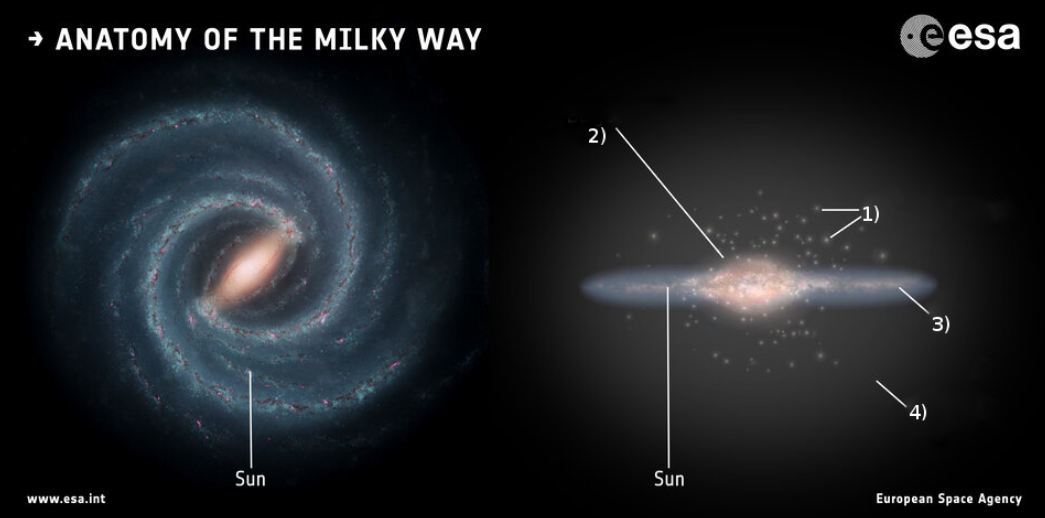
\includegraphics[scale=0.35]{milky.png}}\\
\\
\textbf{1) globular clusters:} Are spheroidal groupings of stars. They can contain from tens of thousands
to many millions of stars. The milky way has more than 150 known globular clustes one of them is Omega 
Centauri.\\
\textbf{2) bulge:} Is the dense central area of a spiral galaxy. The bulge is as well a group of stars 
located at the center of a spiral galaxy.\\
\textbf{3) disk:} Is a flattened, rotating structure, which contains stars, gas and dust. The disk of the
Milky Way has a diameter of about 100,000 light-years and is around 1,000 light-years thick.\\
\textbf{4) halo:} Is a spherical region surrounding the disk. The stars and globular clusters located in
the halo tend to be old.\\
\\
b) Estimate how many revolutions around the center of the Milky Way the sun has already completed during
its lifetime. You can assume, the sun's age to be 4.6 Gyr, while the angular velocity of the sun's orbit
can be computed from the Oort constants by using the equation $A - B = \frac{V_0}{R_0} = \omega$.\\
\\
With the age of the Sun and the angular velocity we can determine the total distance travelled by our
solar system:
\begin{equation*}
  s = V_0 \cdot t
\end{equation*}
The velocity of the Sun is $V_0$ in $\omega = \frac{V_0}{R_0}$, where $R_0$ is the distance from the Sun
to the center of the Milky Way. We can then devide the total distance by the circumference of the circle, 
with the radius of the distance from the Sun to the center of the Milky Way to receive the number of 
revelations made during the lifespan of the Sun:
\begin{equation*}
  \begin{split}
    n &= \frac{s}{2 \pi R_0}\\
      &= \frac{(A - B) \cdot R_0 \cdot t}{2 \pi R_0}
  \end{split}
\end{equation*}
The Oorts constants are: $A = 15.3 \pm 0.4 \text{km} \text{s}^{-1} \text{kpc}^{-1}$ and 
$B = -11.9 \pm 0.4 \text{km} \text{s}^{-1} \text{kpc}^{-1}$. Therfore the angular velocity of the sun
orbiting around the Milky Way is:
\begin{equation*}
  \begin{split}
    \omega &= 15.3 \pm 0.4 \text{km} \text{s}^{-1} \text{kpc}^{-1} - (-11.9 \pm 0.4 \text{km} \text{s}^{-1} \text{kpc}^{-1})\\
    &= 27.2 \pm 0.8 \text{km} \text{s}^{-1} \text{kpc}^{-1}
  \end{split}
\end{equation*}
If we insert that into the equation:
\begin{equation*}
  \begin{split}
    n &= \frac{(A - B) \cdot R_0 \cdot t}{2 \pi R_0}\\
      &= \frac{27.2 \pm 0.8 \text{km} \text{s}^{-1} \text{kpc}^{-1} \cdot t}{2 \pi}\\
      &= \frac{\frac{27.2 \pm 0.8}{3.086 \cdot 10^{16}} \text{kpc} \text{s}^{-1} \text{kpc}^{-1} \cdot t}{2 \pi}\\
      &= \frac{\frac{27.2 \pm 0.8}{3.086 \cdot 10^{16}} \text{s}^{-1} \cdot t}{2 \pi}\\
      &= \frac{\frac{27.2 \pm 0.8}{3.086 \cdot 10^{16}} \text{s}^{-1} \cdot 4.6 \cdot 10^9 yr}{2 \pi}\\
      &= \frac{\frac{27.2 \pm 0.8}{3.086 \cdot 10^{16}} \text{s}^{-1} \cdot 4.6 \cdot 10^9 \cdot 3.154 \cdot 10^7 s}{2 \pi}\\
      &= \frac{\frac{27.2 \pm 0.8}{3.086 \cdot 10^{16}} \text{s}^{-1} \cdot 4.6 \cdot 10^{16} \cdot 3.154 s}{2 \pi}\\
      &= \frac{\frac{27.2 \pm 0.8}{3.086} \text{s}^{-1} \cdot 4.6 \cdot 3.154 s}{2 \pi}\\
      &= \frac{\frac{27.2 \pm 0.8}{3.086} \cdot 4.6 \cdot 3.154}{2 \pi}\\
      &\approx 0.748245 (27.2 \pm 0.8)\\
  n_0 &= 0.748245 (27.2 - 0.8)\\
  n_0 &= 19.753668\\
  n_1 &= 0.748245 (27.2 + 0.8)\\
  n_1 &= 20.95086
  \end{split}
\end{equation*}
Therefore we can estimate our solar system made between 19 and 21 full revelations around the center of
the Milky Way in its lifespan.\\
\\
c) Estimate the distance of the following objects to the disc of the Milky Way: (1) the Globular cluster
M13 ($l = 59.0^{\circ}, b = 40.9^{\circ}$); (2) Orion Nebula ($l = 209.0^{\circ}, b = 19.4^{\circ}$). M13
has a distance of 7 kpc to the Sun, while the Orion Nebula has a distance of 450 pc to the sun. Based on
the position of M13 and the Orion Nebula in the Milky Way, estimate to which galactic component those
objects belong. Justify your answer by taking into account the connection between the distribution of the
gas in the Milky Way and the stellar formation.\\
\\
To make an estimation of the location of the following objects in the Galaxy we can use the following
formula:
\begin{equation*}
 d = d_s \cdot cos(b)
\end{equation*}
where $d$ is the distance from the centre of the disk, $d_s$ is the distance to the Sun and $b$ is the
galactic latitude. Therefore we get:
\begin{equation*}
  \begin{split}
    d_{M13} &= 7 \text{kpc} \cdot cos(40.9^{\circ})\\
            &\approx 5.29097 \text{kpc}\\
            &= 5,290.97 \text{pc}
  \end{split}
\end{equation*}
, and:
\begin{equation*}
  \begin{split}
    d_{ON} &= 450 \text{pc} \cdot cos(19.4^{\circ})\\
           &\approx 424.4502 \text{pc}
  \end{split}
\end{equation*}
Further: within the distance of a few hundered parsec we can say that the object is part of the disk. Is
this threshold breached the object is likely part of the halo.\\
With that in mind we can evaluate our calculations and say that M13 is likely part of the halo and the 
Orion Nebula is likely part of the disk of the Milky Way. After a quick google search I found out that
M13 is not gas rich, while Orion Nebula is. This further supports my assumtion as gas rich clusters are
usually located close to the disk and old gas poor clusters are further away from the disk.

